%!TEX root = document.tex

% Note: activity SAGs can go beyond friends.

%In this section we evaluate the correlation between the conditional
%entropy and size of groups, pages and favourites.

We analyze the informativeness of Activity SAGS by looking at the correlation 
between the size and type of groups, pages and favourites.

Fig \ref{Fig3} shows the relationship between conditional
    entropy and logistic regression weights versus the size of activity
    groups. Here the size of a {\em group}, {\em page} and {\em favorite} 
    is the number of total users in the activity group. 
    For {\em Pages} and {\em Favorites} this is the total number of Facebook users, 
    whether or not they are in the App users' ego network, while for 
    {\em Groups} only the number of users in the App users' ego network is visible to our app.
    Both scatter plots shows that the activity groups of small size can be
    highly predictive (low conditional entropy or weights that deviate
    extremely from zero) whereas large groups are rarely predictive.

In Fig~\ref{Fig4} we plot the average conditional entropy of the top
    10\% of features cumulative up to the size of the activity group given on the
    x-axis; this allows us to determine the marginal contribution of
    larger groups to the average conditional entropy as larger groups
    are incrementally added in.  This graph 
    distinctly shows that the small sizes of groups, pages and favourites
    have low average conditional entropy that transitions sharply to a
    higher average once a size threshold has been met.  From 
    Fig~\ref{Fig4} we can infer that the group sizes up to 50 and
    page/favourite sizes up to $10^{5}$ are most predictive.

%{\bf TODO: make this consistent with earlier discussion regarding persistence,
%temporally sychronized.}

 We also analyze predictiveness of favourites by categories in
    Fig~\ref{Fig5}, where the favorite categories are obtained from Facebook API.  
    %It shows that SAGs consisting of shared interests,
    %activity, television, and books are on average most predictive, while 
    %music, movies, favourite teams, sports and athletes are on average
    %least predictive.  
    We can see that contents in the ``long-tail'', i.e.,  
    having a large number of occurrences far from the most popular choices, 
    tend to have be the most predictive affinities. Examples of these include
    music, books, movies. On the contrary, generic affinities (e.g. interests) and 
    those with a smaller number of choices (e.g. sports or fav-teams) 
    tend to be less predictive. 
    %While favourite teams, sports and athletes may be
    %too focused to offer much predictiveness vs. the other more diverse
    %categories, it is interesting that movies and music favourites
    %are not very predictive on average.  This may have to do with the fact that
    %these are typically ephemeral favourites that may be heavily influenced
    %by popularity as opposed to true personal preference.
%\end{itemize}

%In Fig~\ref{Fig4} we plot the average conditional entropy of top
%    10\% features cumulative over the size of activity group. It
%    distinctly shows that the small sized group, pages and favourites
%    have low average conditional entropy. Furthermore, it explains
%    average conditional entropy decreases as size increases. From the
%    figure \ref{Fig4} we can infer that the group size upto 50 and
%    page/favourite size upto $10^{5}$ can be highly predictive.
%
%We also analyze predictiveness of favourites by categories in
%    Fig \ref{Fig5}. It shows that television, books, music and movies
%    are predictive whereas favourite teams, sports and athletes are
%    less predictive.
%\end{itemize}

%\TODO{add a table of top 5-10 groups/pages/favs}

\begin{table*}[tbp!]
\centering
\begin{tabular}{| >{\small}l | >{\small}r | >{\small}r |}
\hline
\textbf{Top Groups} & \textbf{Top Pages} & \textbf{Top Favourites} \\
\hline
%Heavy Metal - Australian Capital Territory & Avascular Necrosis & Avascular Necrosis \\
Heavy Metal - (city name) & Avascular Necrosis & Avascular Necrosis \\
Stephen Conroy Should Not Filter Our Internet & Assidian & Tortured \\
Silicone Stripper & Tortured & Elysian \\
Hardcore dancing is not moshing & Elysian & Anno Domini \\
%Metal bands come to Canberra cause I'm sick of... & Darker Half & Hellbringer \\
Metal bands come to (city name) cause I'm sick of... & Darker Half & Hellbringer \\
%Canberra Rock Gigs & Johnny Roadkill & Johnny Roadkill \\
(city name) Rock Gigs & Johnny Roadkill & Johnny Roadkill \\
%Let's Mosh - Canberra metal radio show - 2XX 9 & Anno Domini & Darker Half \\
Let's Mosh - (city name) metal radio show - 2XX 9 & Anno Domini & Darker Half \\
Bring Steel Panther to Australia & Billy Madison & Bane Of Isildur \\
%Canberra Death/Heavy Metal Appreciation & Hellbringer & Katabasis \\
(city name)  Death/Heavy Metal Appreciation & Hellbringer & Katabasis \\
Robert The Bruce (Band) & Metalocalypse & Aeon of Horus \\
\hline
\end{tabular}
\caption{Top 10 Groups/Pages/Favourites ranked by Conditional Entropy. The city name where our institution and many Facebook users resides is anonymized.}
\label {table:topGroupPagesFavs}
\end{table*}

%%%%%%%%%%%%%%%%%%%%%%%%%%%%%%%%%%%%%%%%%%%%%%%%%%%%%%%%%%%%%%%%%%%%%%%%%%%
\begin{figure*}[tbp!]
\centering
\begin{tabular}{ccc}
\begin{tabular}{ccc}
\subfloat[Fig:][]{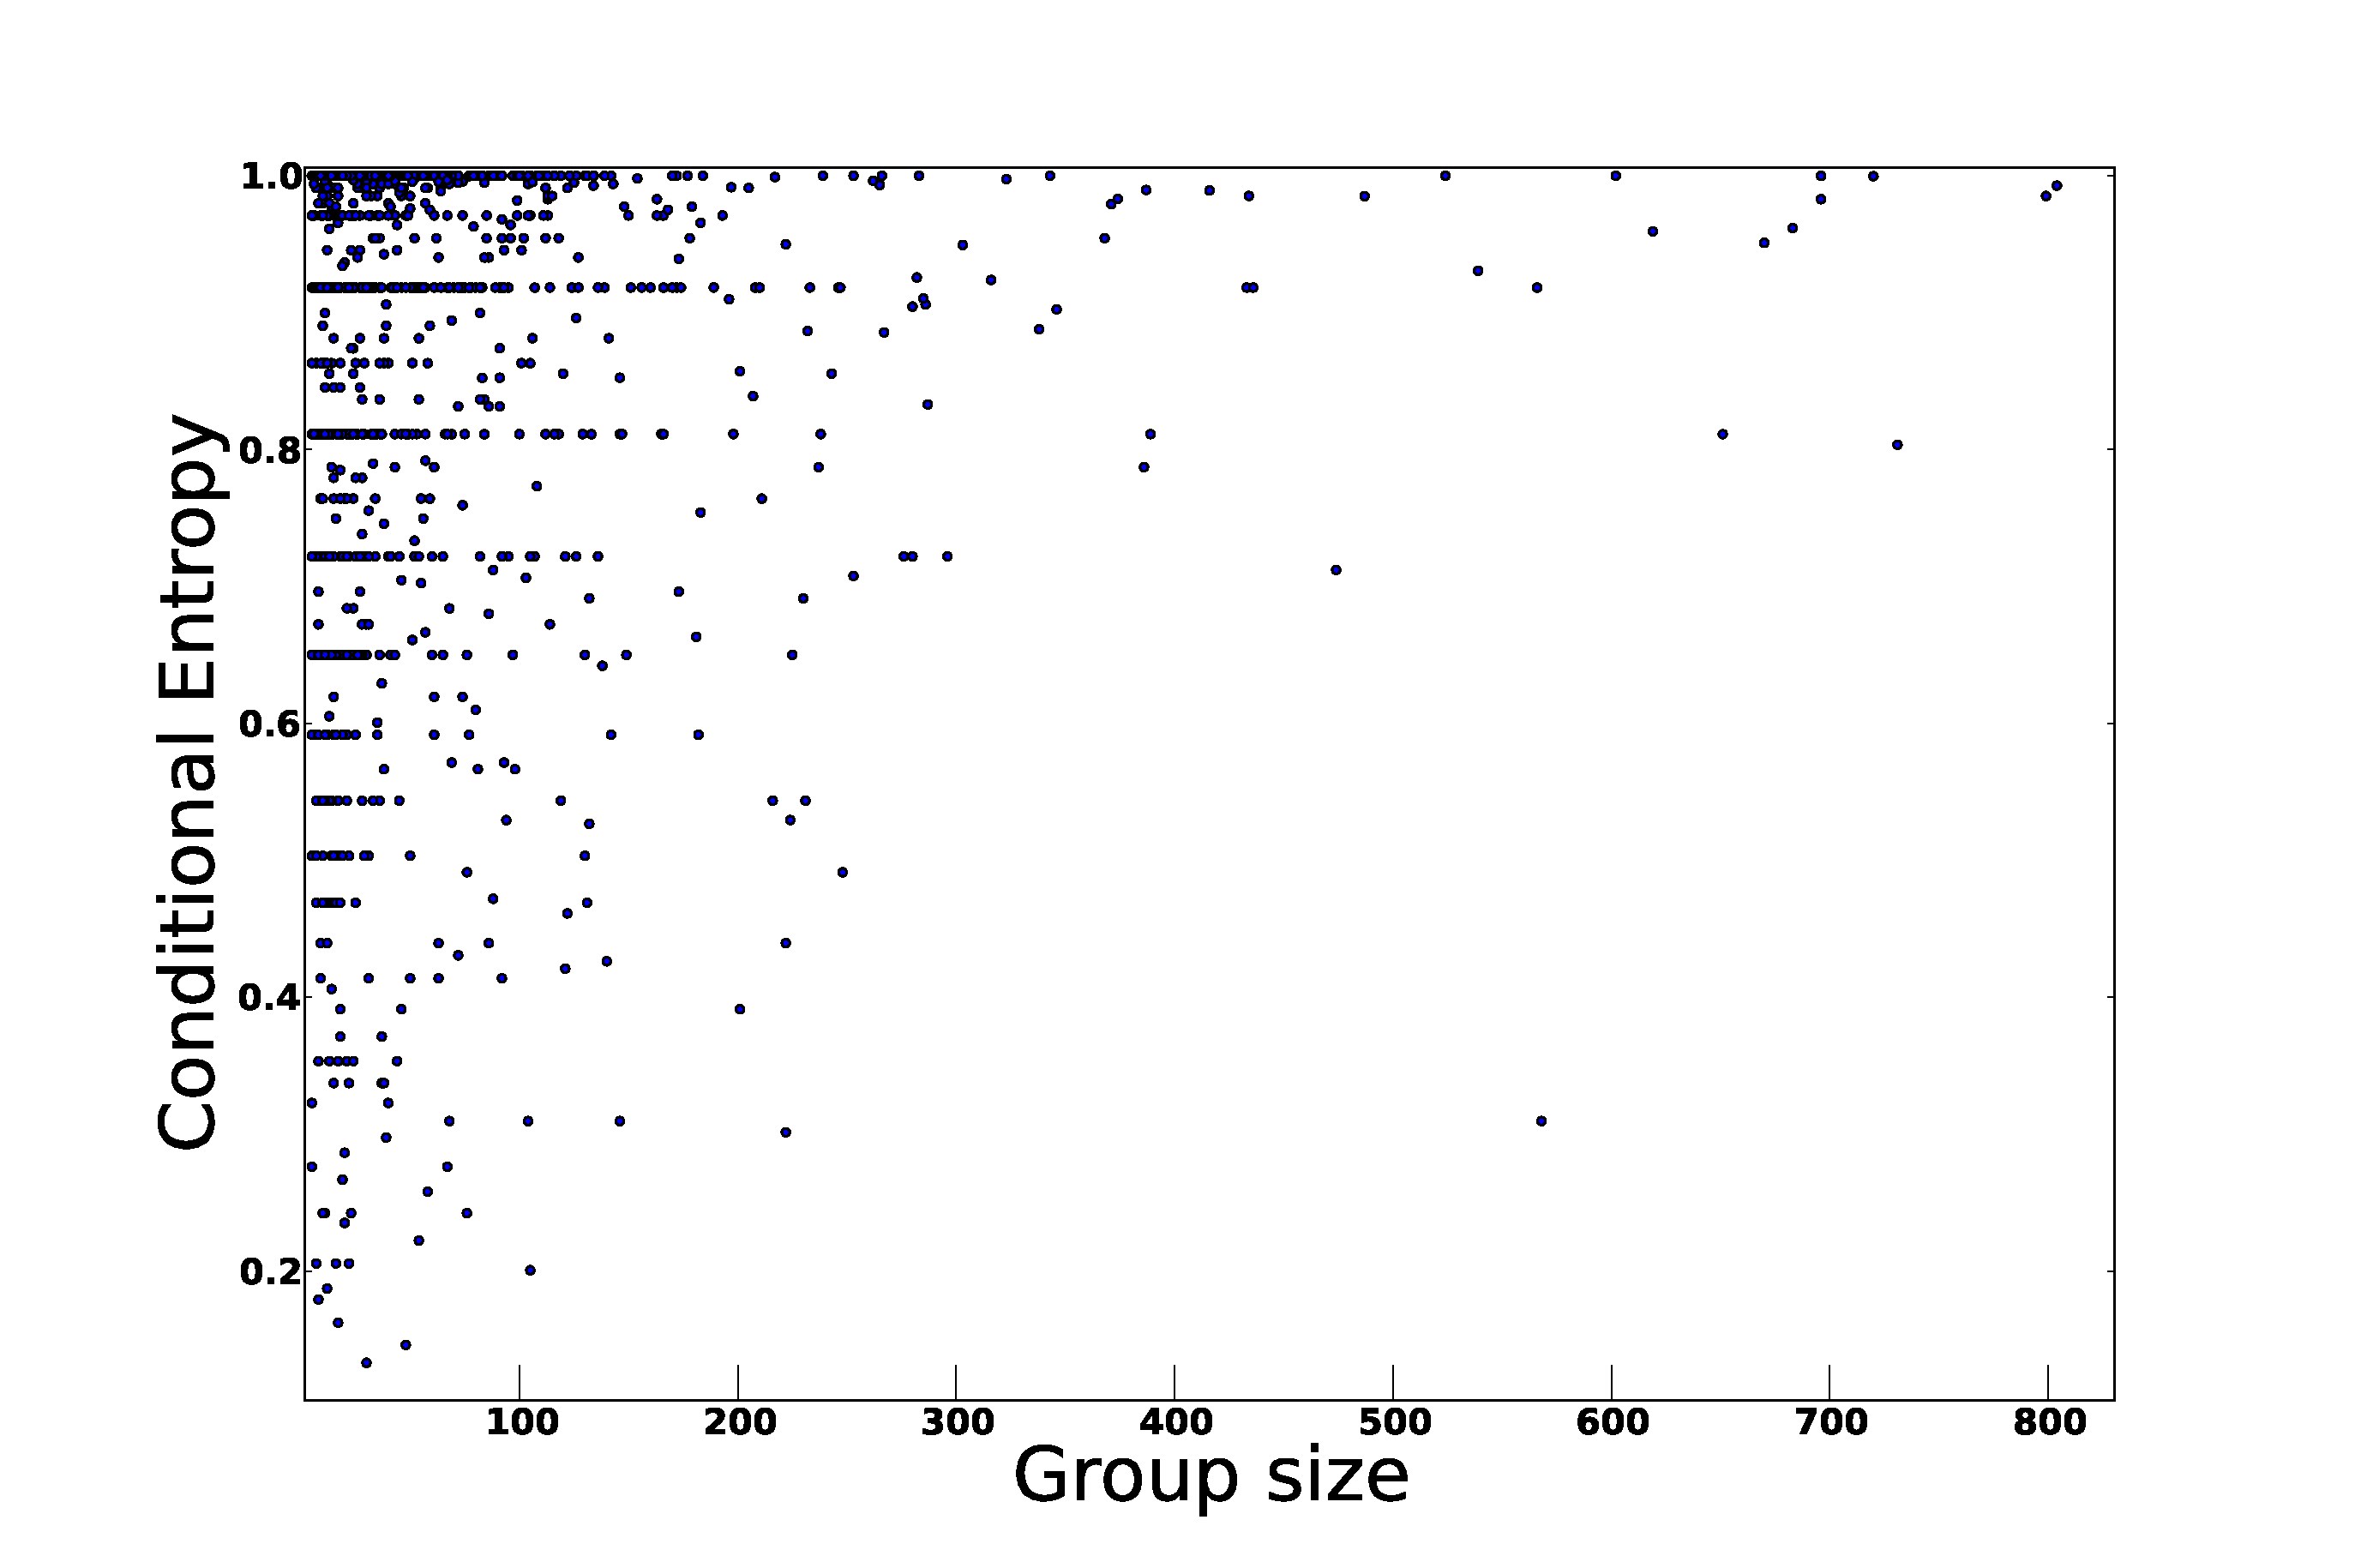
\includegraphics[width=45mm, height=35mm]{data/plots/new/CEvsGroupSize.eps}}
\subfloat[Fig:][]{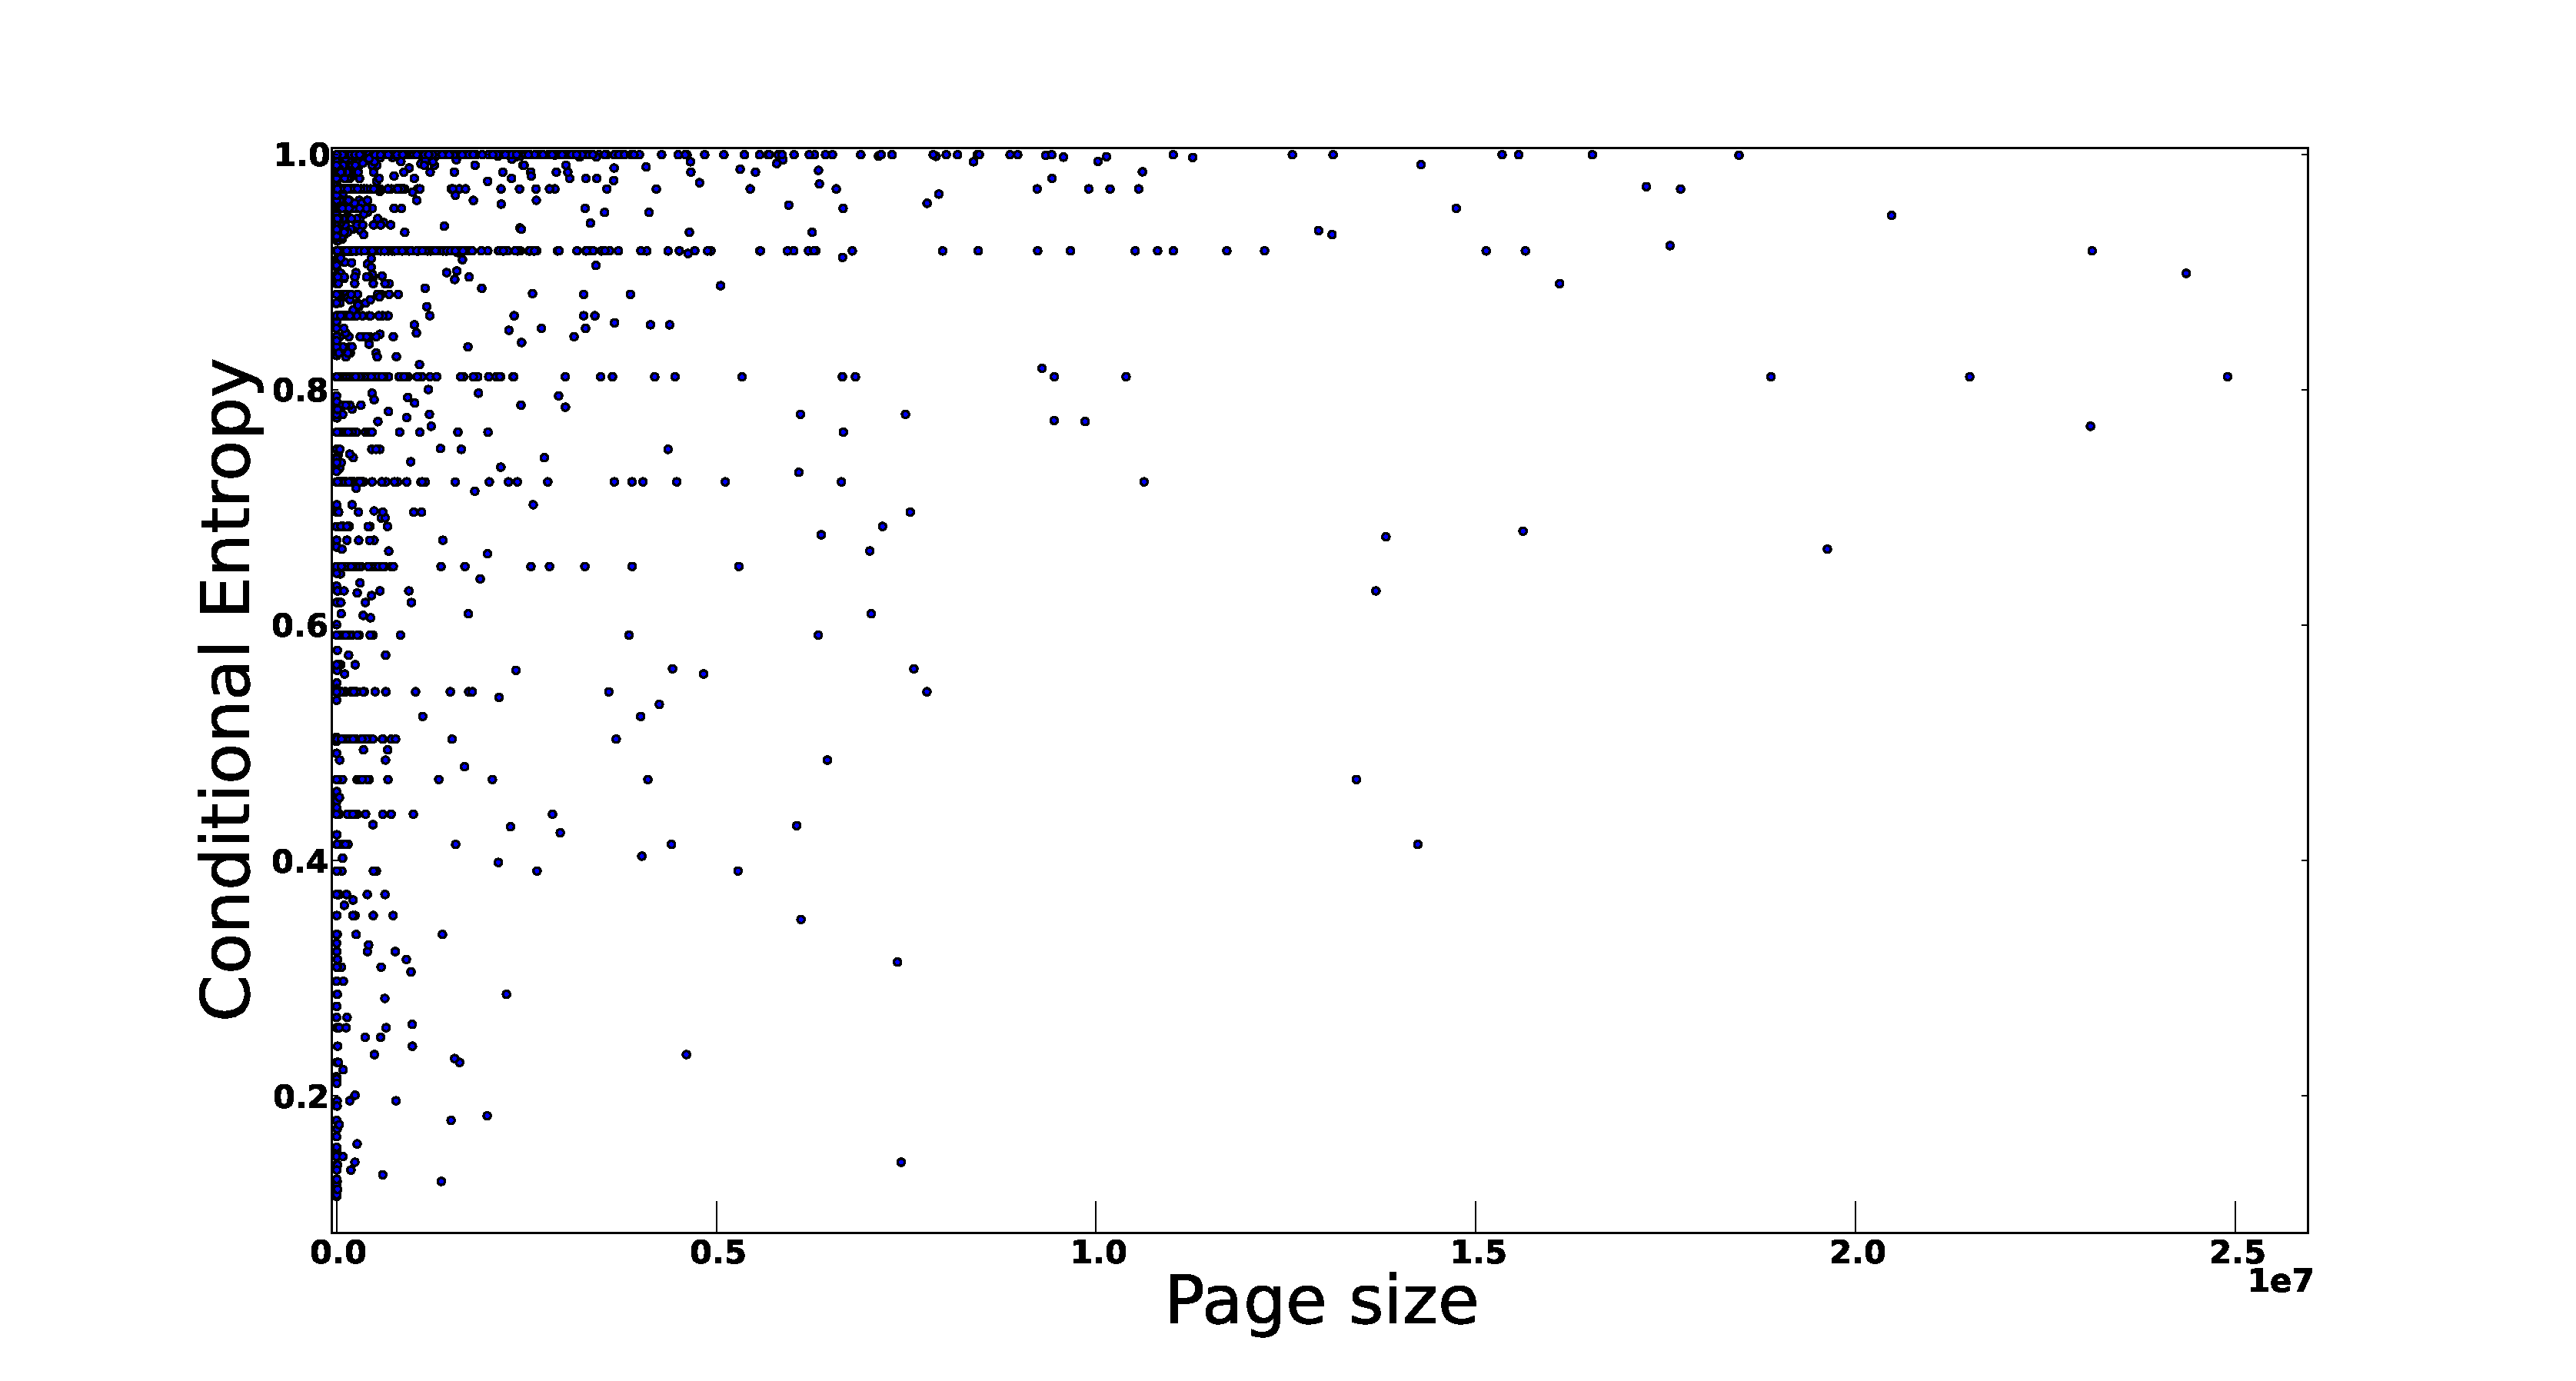
\includegraphics[width=45mm, height=35mm]{data/plots/new/CEvsPageSize.eps}}
\subfloat[Fig:][]{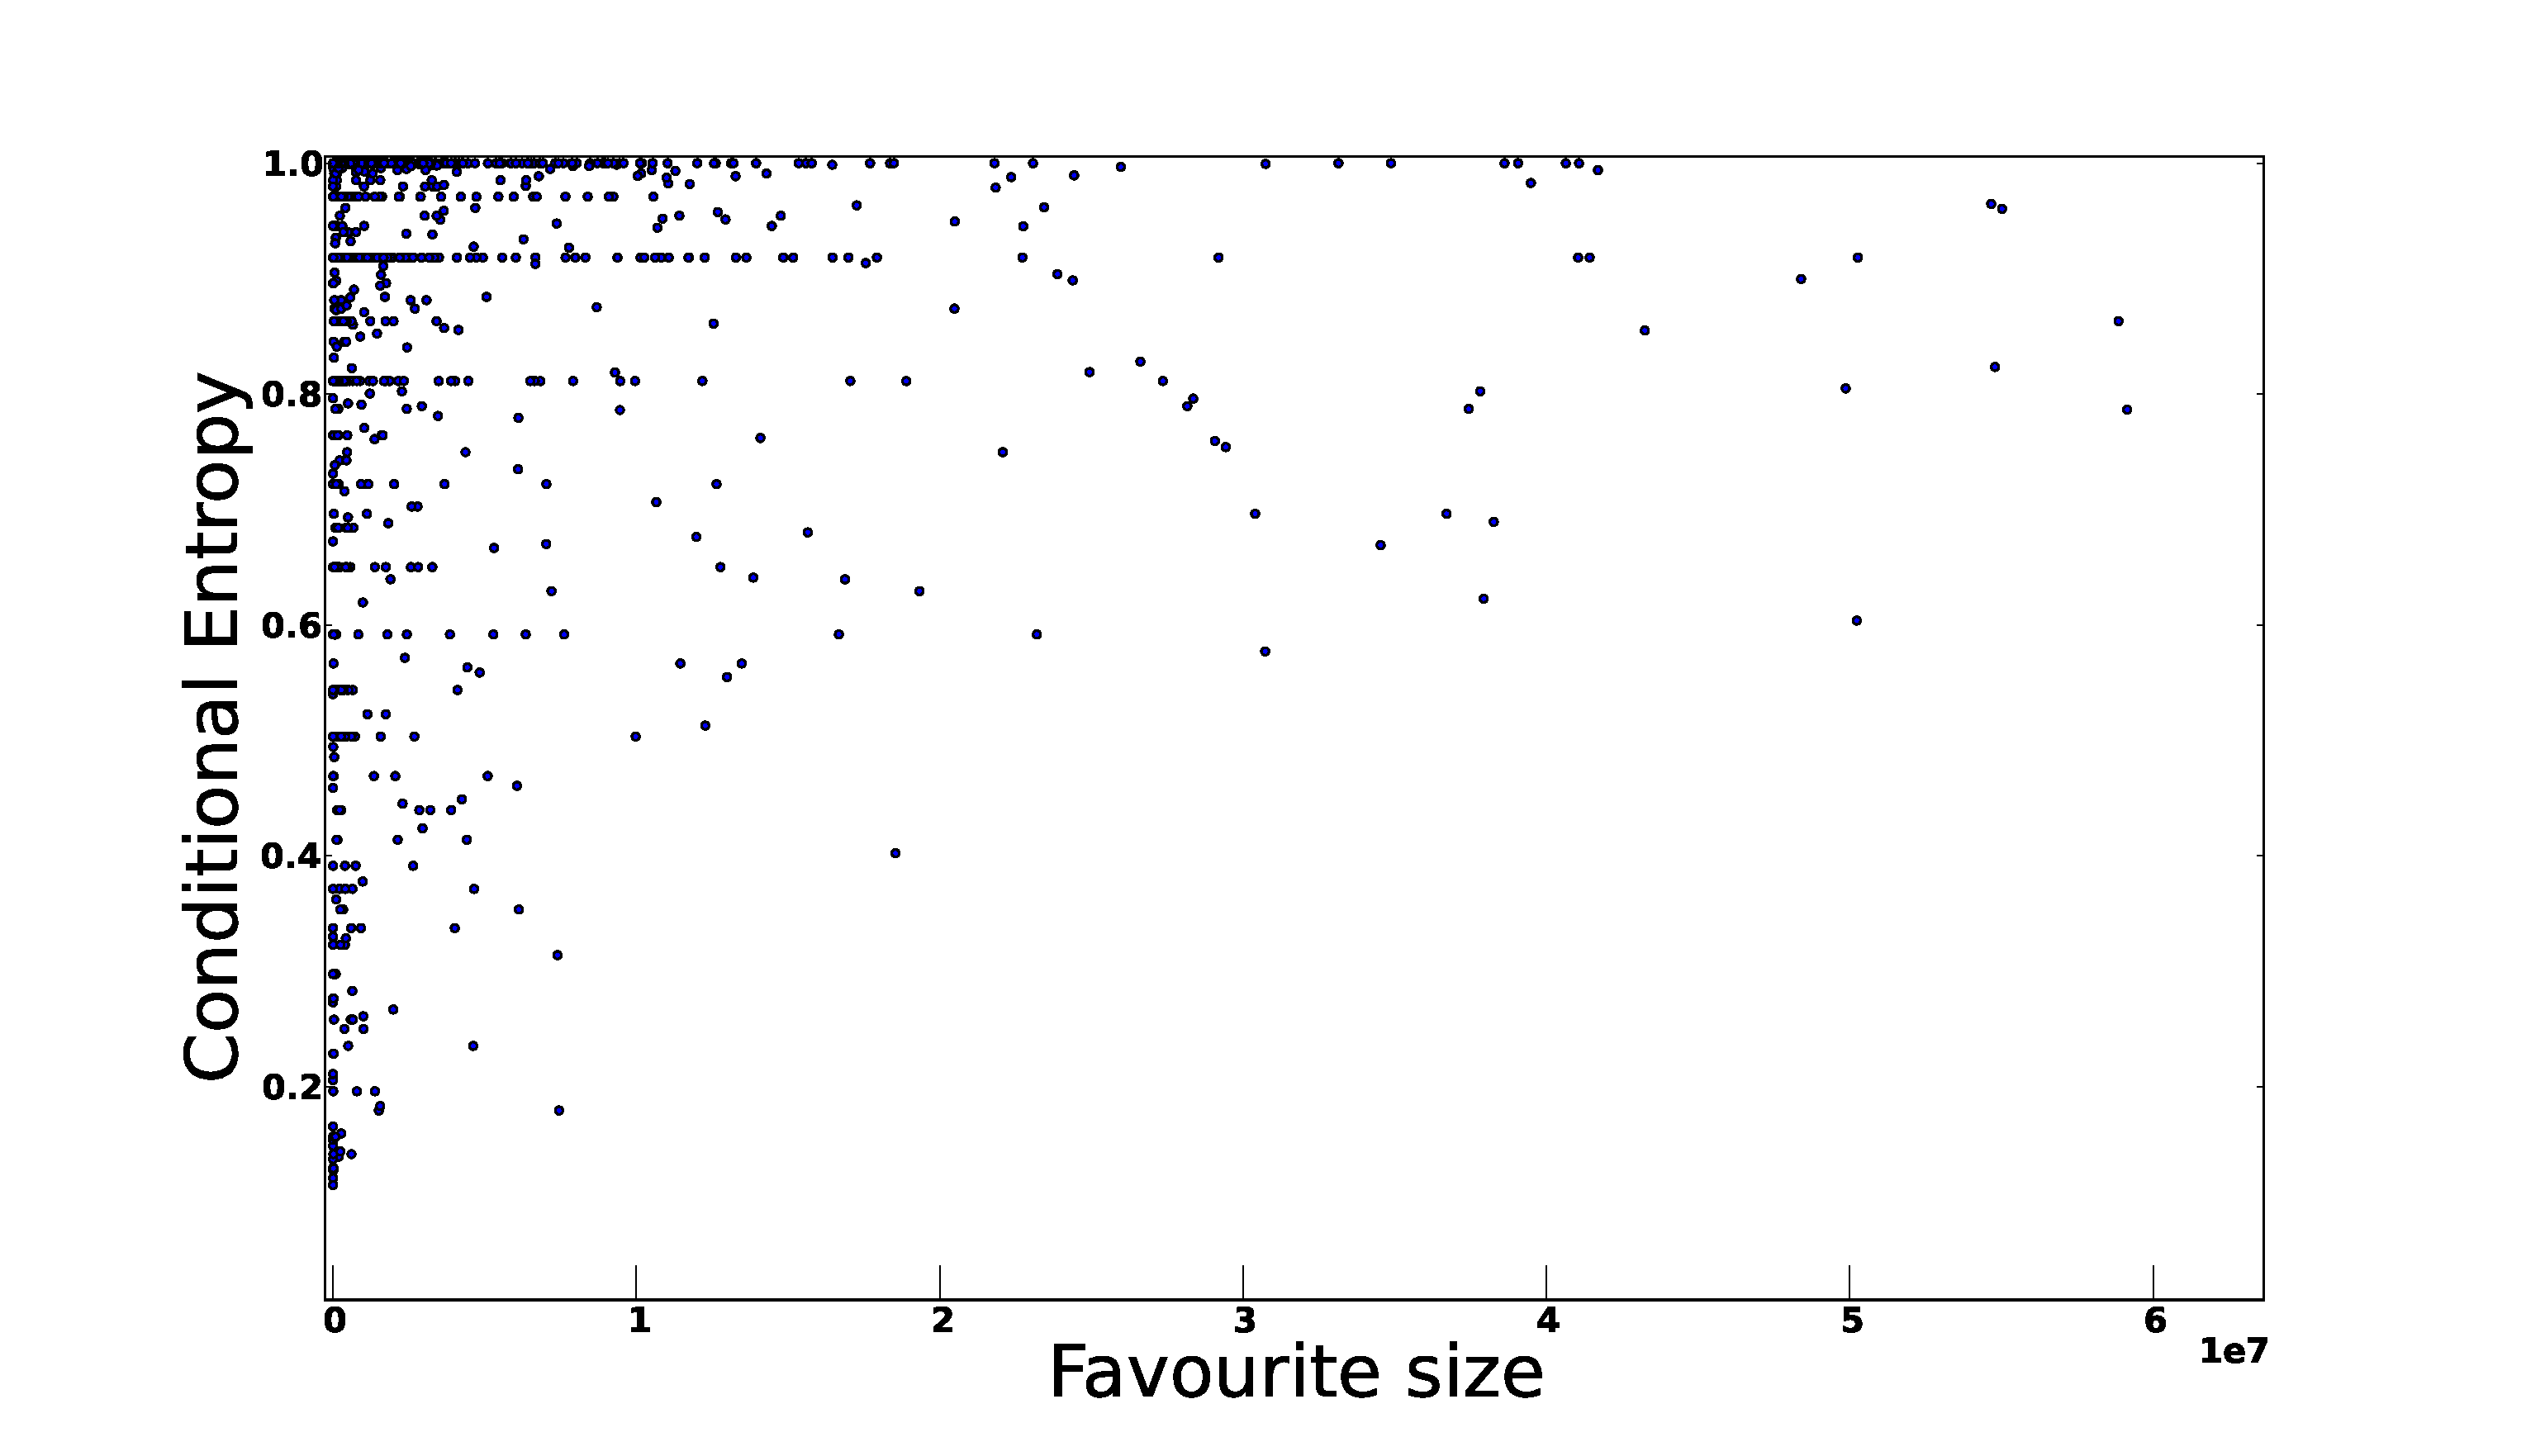
\includegraphics[width=45mm, height=35mm]{data/plots/new/CEvsFavSize.eps}} \\
\subfloat[Fig:][]{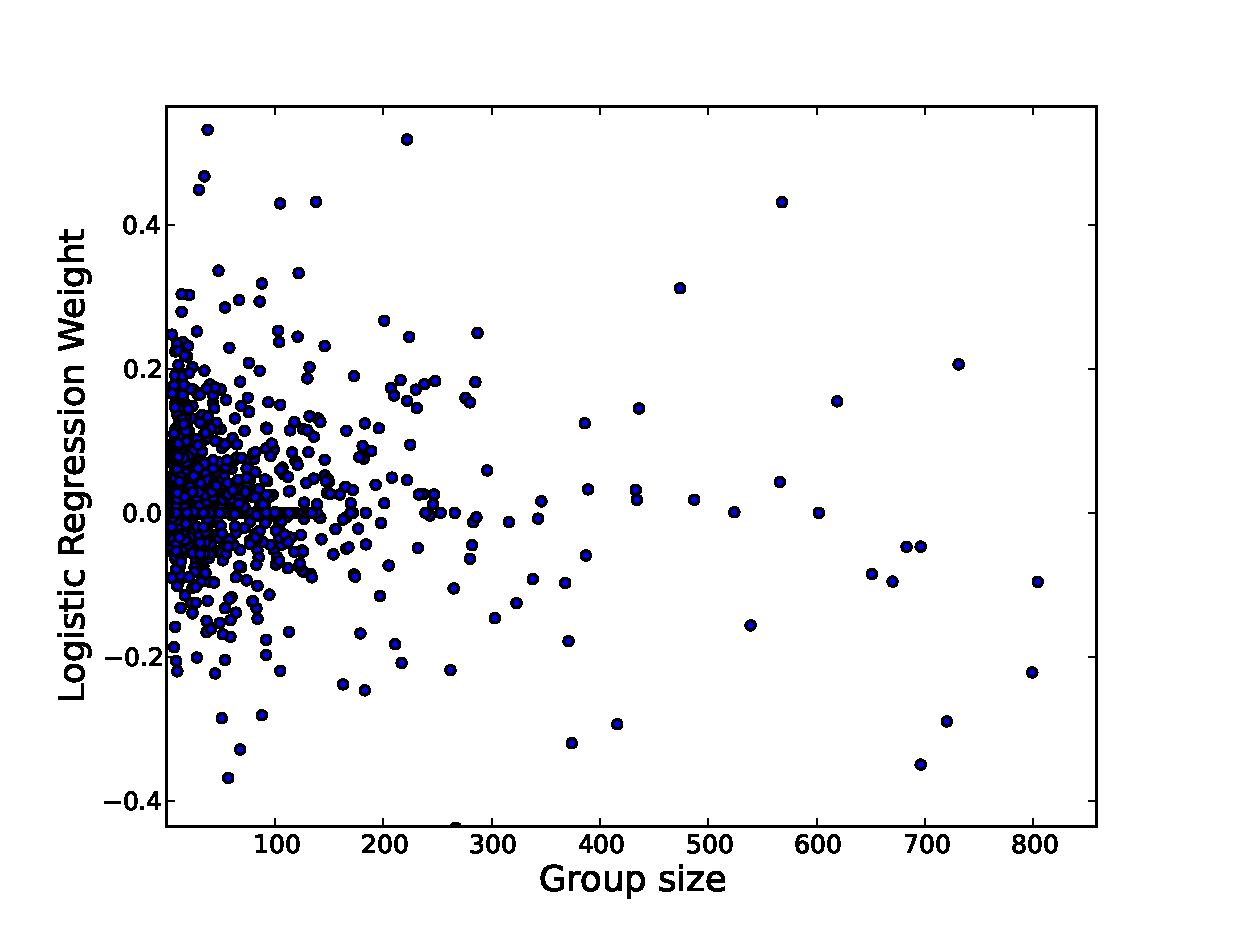
\includegraphics[width=45mm, height=35mm]{data/plots/new/LRweightvsGroupSize.eps}}
\subfloat[Fig:][]{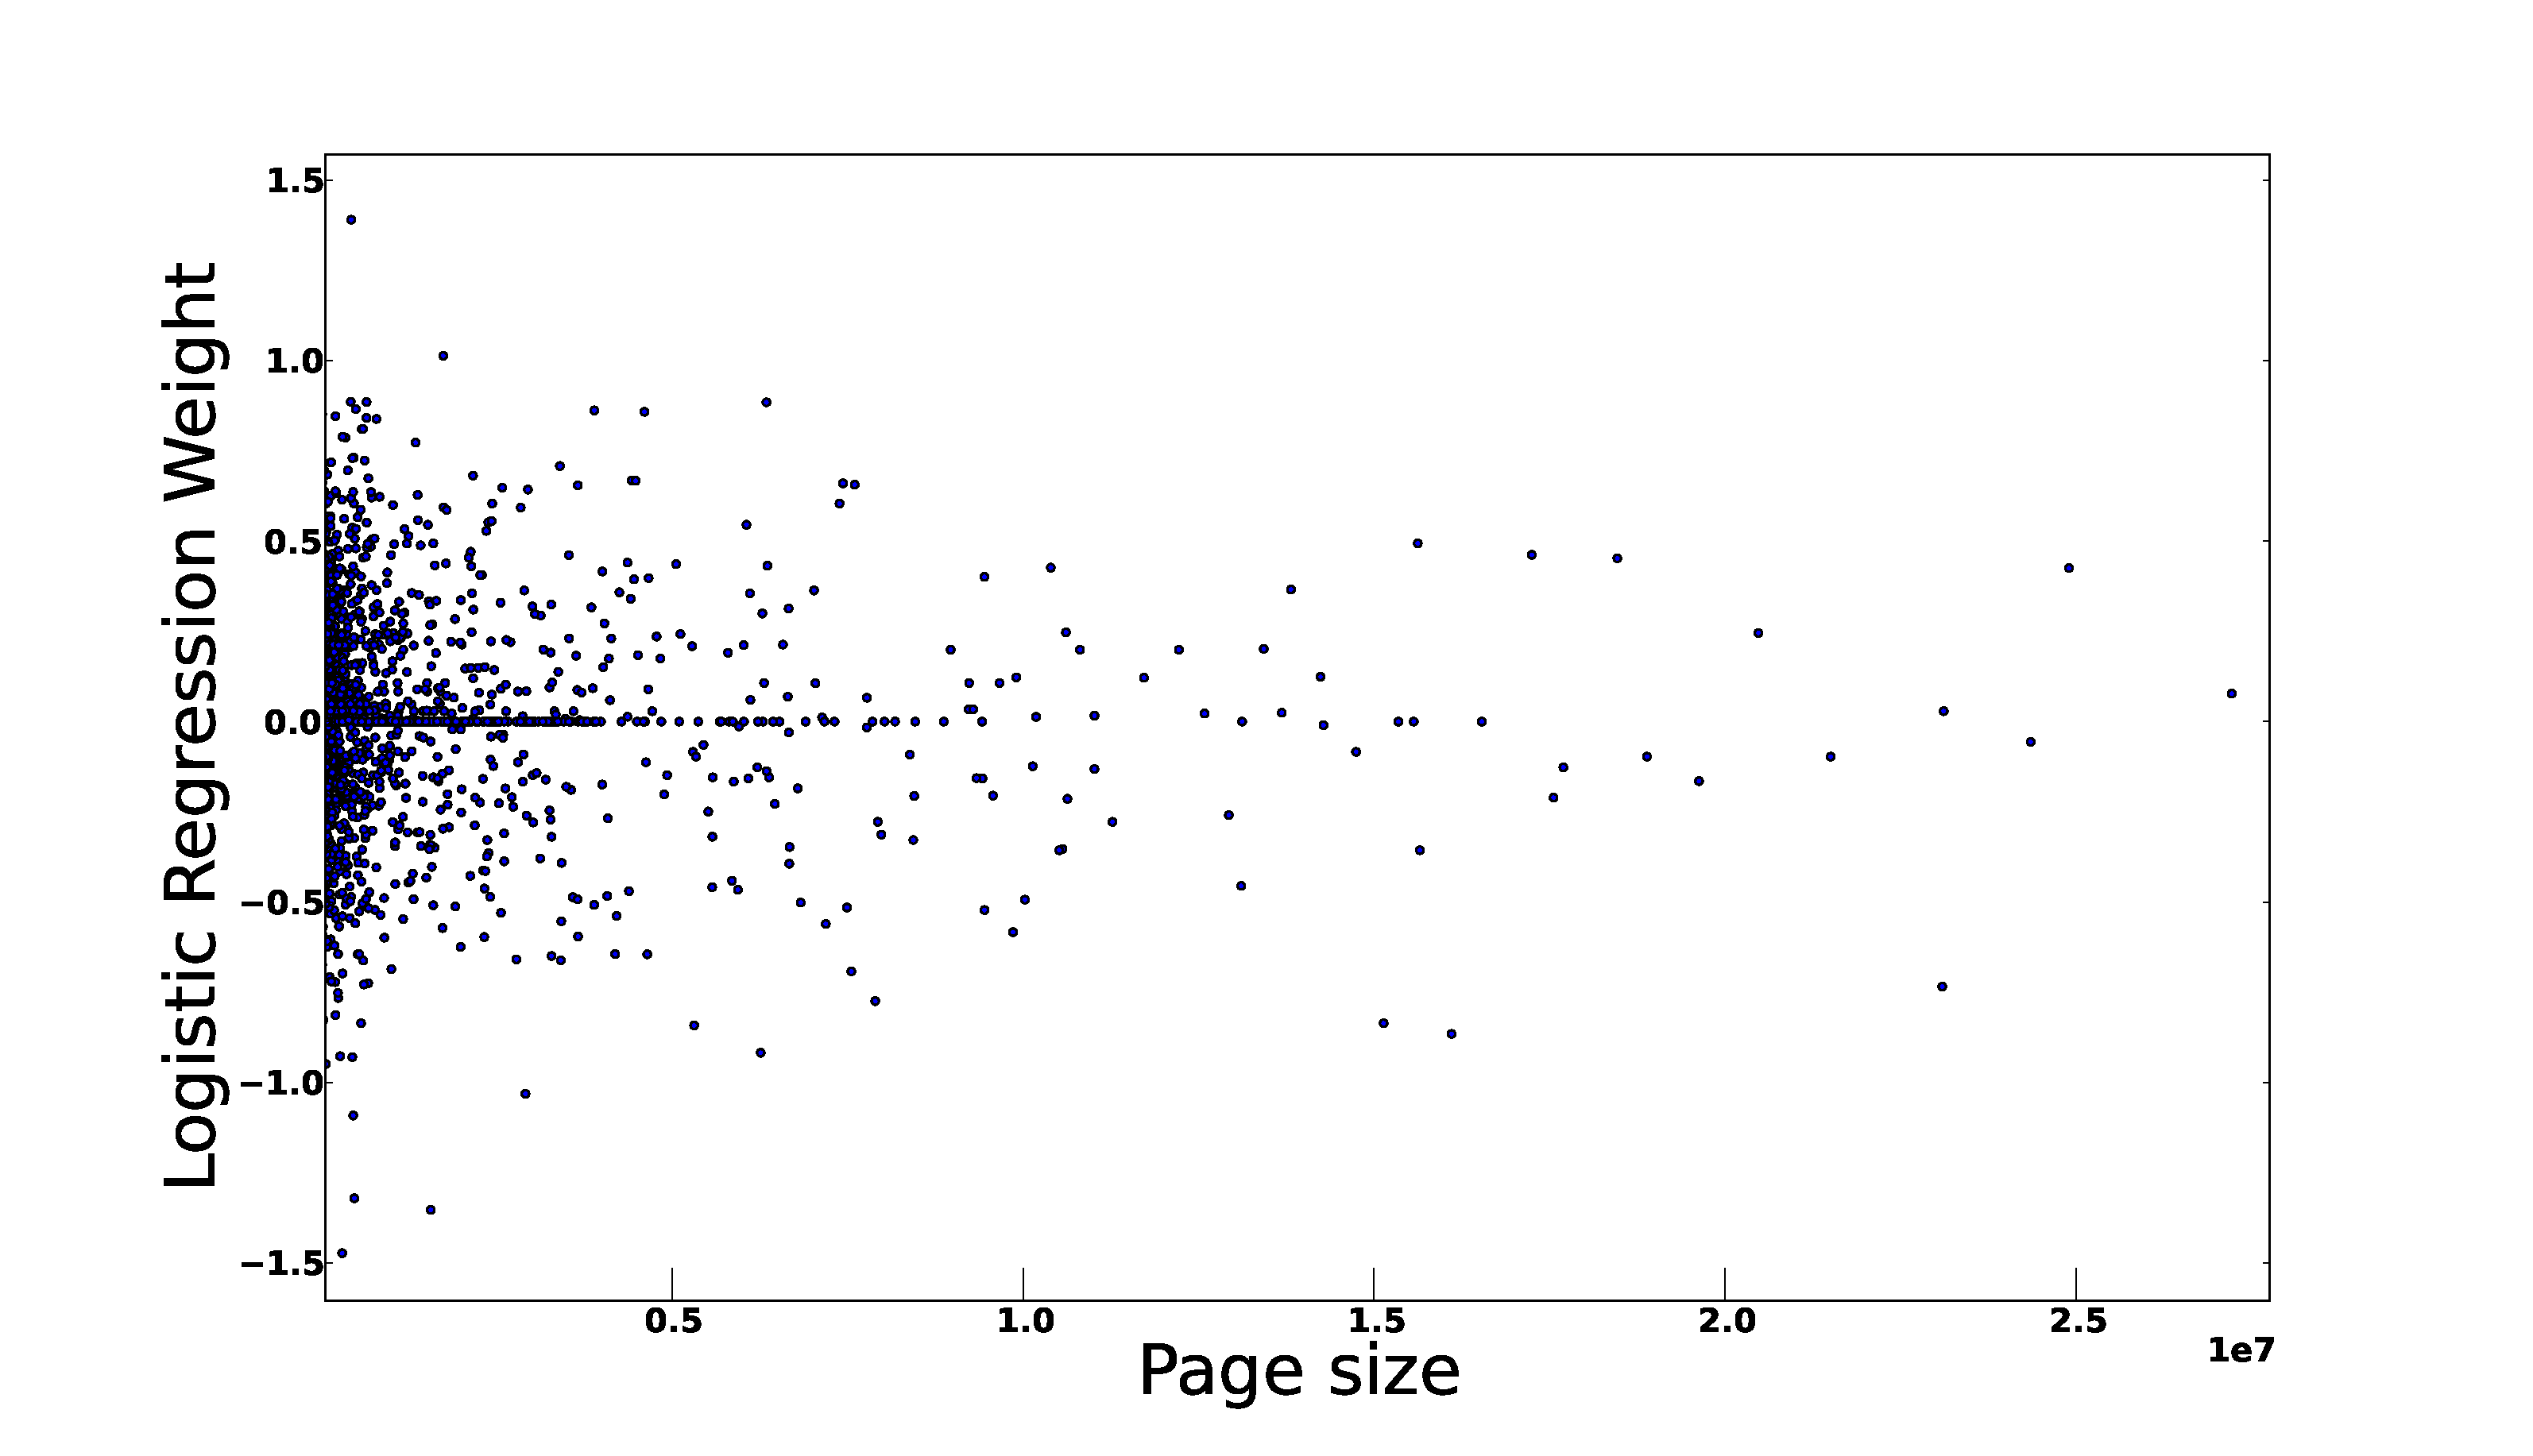
\includegraphics[width=45mm, height=35mm]{data/plots/new/LRweightvsPageSize.eps}}
\subfloat[Fig:][]{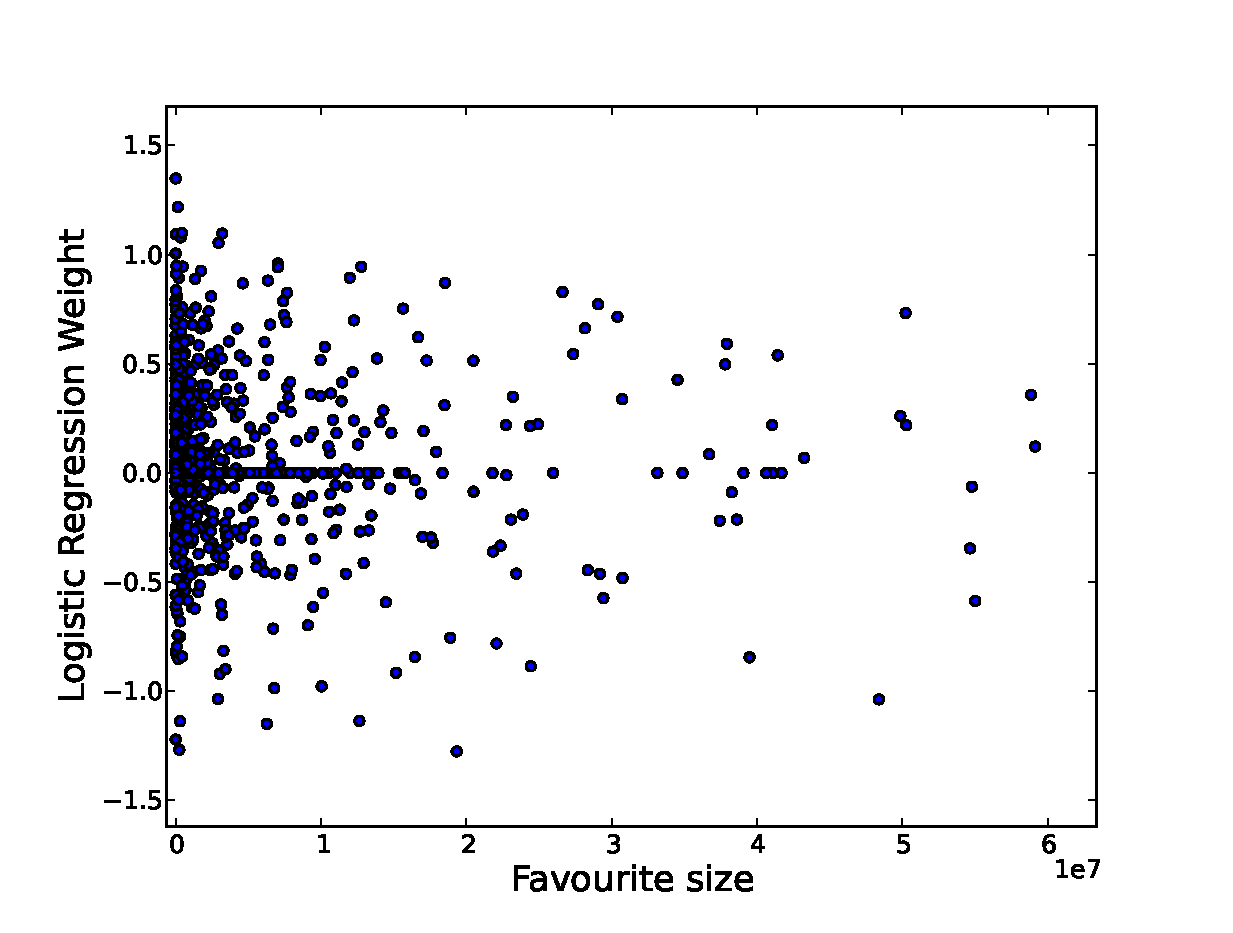
\includegraphics[width=45mm, height=35mm]{data/plots/new/LRweightvsFavSize.eps}} \\
\end{tabular}
\end{tabular}
\caption {Conditional entropy vs size (a-c); logistic regression feature weights vs size (d-f) }
\label{Fig3}
\end{figure*}
%%%%%%%%%%%%%%%%%%%%%%%%%%%%%%%%%%%%%%%%%%%%%%%%%%%%%%%%%%%%%%%%%%%%%%%%%%%

%%%%%%%%%%%%%%%%%%%%%%%%%%%%%%%%%%%%%%%%%%%%%%%%%%%%%%%%%%%%%%%%%%%%%%%%%%%
\begin{figure*}[tbp!]
\centering
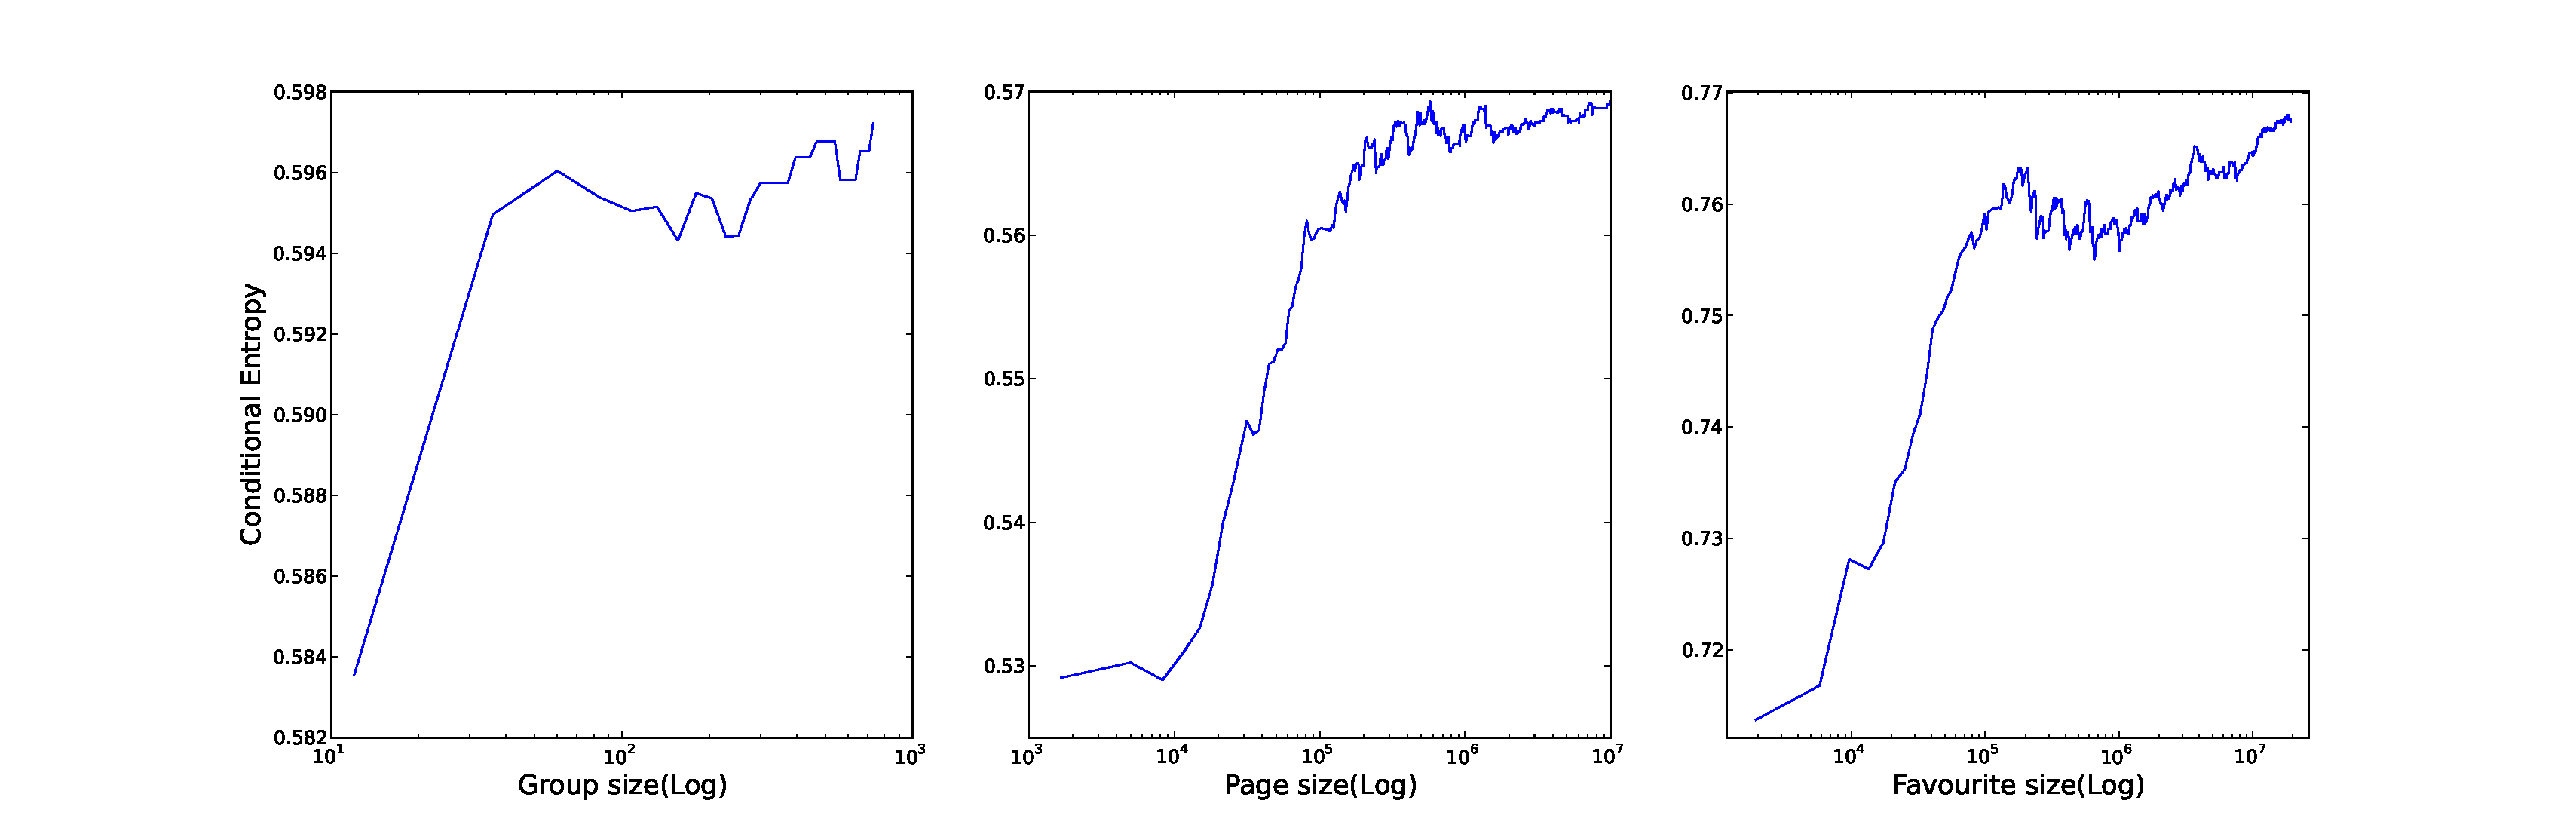
\includegraphics[scale=0.28]{data/plots/cumulativeEntropy/cumulative.eps}
\caption{Average conditional entropy of top 10\% groups, pages and favourites features cumulative over the size }
\label{Fig4}
\end{figure*}
%%%%%%%%%%%%%%%%%%%%%%%%%%%%%%%%%%%%%%%%%%%%%%%%%%%%%%%%%%%%%%%%%%%%%%%%%%%

%%%%%%%%%%%%%%%%%%%%%%%%%%%%%%%%%%%%%%%%%%%%%%%%%%%%%%%%%%%%%%%%%%%%%%%%%%%
\begin{figure*}[tbp!]
\centering
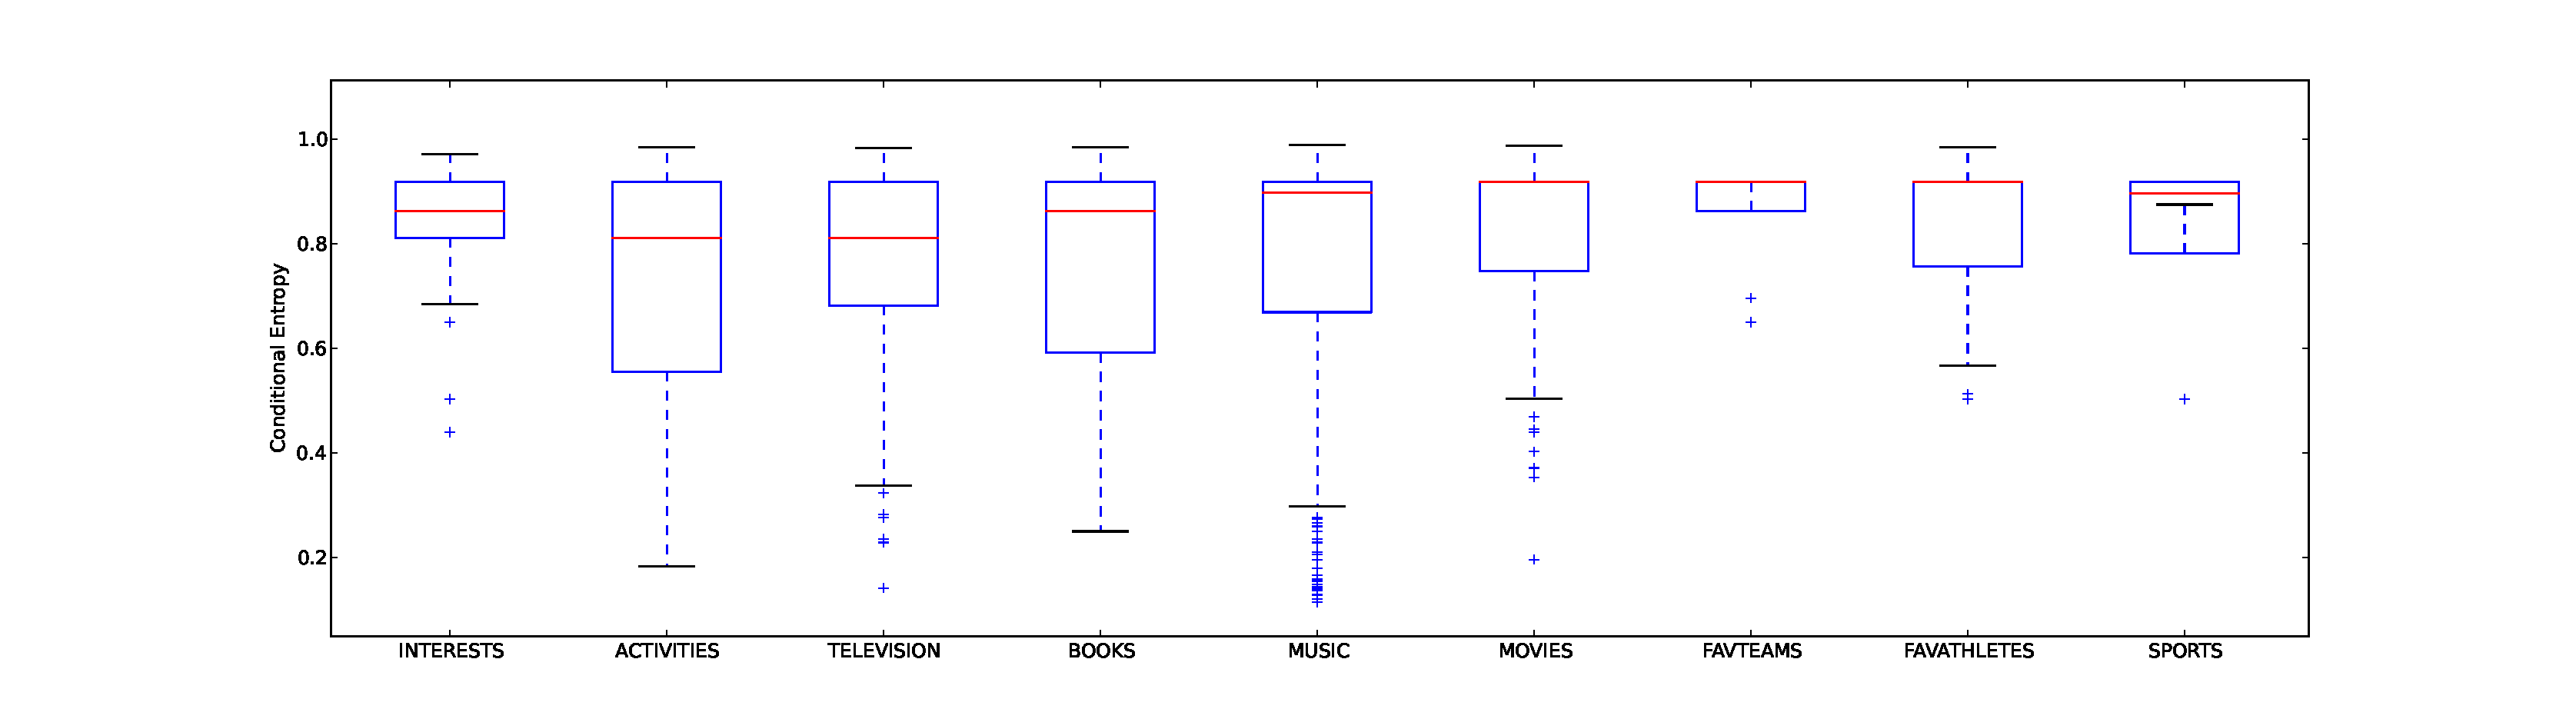
\includegraphics[width=180mm, height=40mm]{data/plots/boxPlots/CEvsFavTypes.eps}
\caption{Conditional entropy for top 1000 favourites breakdown by categories}
\label{Fig5}
\end{figure*}
%%%%%%%%%%%%%%%%%%%%%%%%%%%%%%%%%%%%%%%%%%%%%%%%%%%%%%%%%%%%%%%%%%%%%%%%%%%
